\documentclass[final,5p,times,twocolumn]{elsarticle}

%%%%%%%%%%%%%%%%%%%%%%%%%%%%%%%%%%%%%%%%%%%%%%%%%%%%%%%%%%%%%%%%%%%%%%%%%%%%%%%
% DRAFT v1 -- content filled from provided sources (photos + measurement graphs)
% Format: Elsevier two-column journal layout (Journal of Systems Architecture)
% "TBD" = data not yet available; to be filled by the authors.
%%%%%%%%%%%%%%%%%%%%%%%%%%%%%%%%%%%%%%%%%%%%%%%%%%%%%%%%%%%%%%%%%%%%%%%%%%%%%%%

\usepackage{amsmath,amssymb}
\usepackage{booktabs}
\usepackage{multirow}
\usepackage{array}
\usepackage{float}
\usepackage{algorithm}
\usepackage{algpseudocode}
\usepackage{hyperref}
\usepackage{xcolor}
\usepackage{textcomp}
\usepackage{siunitx}
\usepackage{url}
\usepackage{graphicx}

\journal{Journal of Systems Architecture}

%%%%%%%%%%%%%%%%%%%%%%%%%%%%%%%%%%%%%%%%%%%%%%%%%%%%%%%%%%%%%%%%%%%%%%%%%%%%%%%
% Blank writing area command (kept for still-empty placeholders)
%%%%%%%%%%%%%%%%%%%%%%%%%%%%%%%%%%%%%%%%%%%%%%%%%%%%%%%%%%%%%%%%%%%%%%%%%%%%%%%
\newcommand{\writinggap}[1][2.8cm]{%
\vspace{#1}
}
% Marker for text that still needs author input / data
\newcommand{\todo}[1]{\textcolor{red}{[#1]}}

% No bold anywhere in the document: make the bold series resolve to medium weight.
\renewcommand{\bfdefault}{\mddefault}

\begin{document}

\begin{frontmatter}

%%%%%%%%%%%%%%%%%%%%%%%%%%%%%%%%%%%%%%%%%%%%%%%%%%%%%%%%%%%%%%%%%%%%%%%%%%%%%%%
% TITLE
%%%%%%%%%%%%%%%%%%%%%%%%%%%%%%%%%%%%%%%%%%%%%%%%%%%%%%%%%%%%%%%%%%%%%%%%%%%%%%%
\title{
An Ethernet-Enabled Customizable Neural Inference Framework
on Low-Cost FPGA SoC for High-Frequency Trading
}

%%%%%%%%%%%%%%%%%%%%%%%%%%%%%%%%%%%%%%%%%%%%%%%%%%%%%%%%%%%%%%%%%%%%%%%%%%%%%%%
% AUTHORS
%%%%%%%%%%%%%%%%%%%%%%%%%%%%%%%%%%%%%%%%%%%%%%%%%%%%%%%%%%%%%%%%%%%%%%%%%%%%%%%
\author{%
\centering
{\large Assoc. Prof. Dr. Baykal Sarıoğlu}\\[1pt]
{\itshape Advisor}\\[10pt]
\begin{tabular}{c@{\hspace{2.6cm}}c}
Mustafa Alper Ilık & Ahmet Batuhan Özkaner \\[1pt]
{\footnotesize alper.ilik@bilgiedu.net} & {\footnotesize ahmet.ozakner@bilgiedu.net}
\end{tabular}\\[8pt]
{\normalsize Department of Electrical and Electronics Engineering,
Istanbul Bilgi University, Istanbul, T\"urkiye}%
}

%%%%%%%%%%%%%%%%%%%%%%%%%%%%%%%%%%%%%%%%%%%%%%%%%%%%%%%%%%%%%%%%%%%%%%%%%%%%%%%
% ABSTRACT
%%%%%%%%%%%%%%%%%%%%%%%%%%%%%%%%%%%%%%%%%%%%%%%%%%%%%%%%%%%%%%%%%%%%%%%%%%%%%%%
\begin{abstract}
High-frequency trading (HFT) requires not only accurate decisions but also
predictable, ultra-low decision latency, which is difficult to guarantee on
general-purpose CPUs because of operating-system scheduling, memory hierarchy
effects, and software-stack jitter. This work presents an Ethernet-enabled,
\emph{customizable} neural-inference framework embedded entirely in the
programmable logic of a low-cost Xilinx Zynq-7000 SoC. The processing system
(PS) handles packet reception, feature preparation, and control, while a
fully hardware multi-layer perceptron (MLP) ($40\!\rightarrow\!64\!\rightarrow
\!32\!\rightarrow\!16\!\rightarrow\!3$) performs inference in the programmable
logic (PL). Feature vectors are streamed to the PL through AXI-DMA / AXI-Stream,
and the model is deployed in $Q8.8$ fixed-point format so that a Python-trained
network can be regenerated and re-embedded without redesigning the datapath.
On a Zynq-7000 the design uses \SI{87.3}{\percent} of the DSP slices and
\SI{27.3}{\percent} of the LUTs at \SI{2.78}{\watt}, closes timing at
\SI{125}{\mega\hertz} (WNS \SI{0.118}{\nano\second}), and performs the pure
hardware inference in under \SI{1}{\micro\second}. The FPGA fixed-point model
reproduces the floating-point accuracy within $\approx\!0.2\%$. Because the
feature set, network shape, fixed-point format, and decision classes are all
configurable, the system is best described as a reusable FPGA-embedded AI
inference framework, demonstrated here on an HFT decision task.
\end{abstract}

%%%%%%%%%%%%%%%%%%%%%%%%%%%%%%%%%%%%%%%%%%%%%%%%%%%%%%%%%%%%%%%%%%%%%%%%%%%%%%%
% KEYWORDS
%%%%%%%%%%%%%%%%%%%%%%%%%%%%%%%%%%%%%%%%%%%%%%%%%%%%%%%%%%%%%%%%%%%%%%%%%%%%%%%
\begin{keyword}
FPGA \sep
High-Frequency Trading \sep
Neural Network Inference \sep
Ethernet \sep
Zynq-7000 \sep
Hardware/Software Co-Design \sep
Low-Latency Systems \sep
Fixed-Point Arithmetic
\end{keyword}

\end{frontmatter}

%%%%%%%%%%%%%%%%%%%%%%%%%%%%%%%%%%%%%%%%%%%%%%%%%%%%%%%%%%%%%%%%%%%%%%%%%%%%%%%
\section{Introduction}
%%%%%%%%%%%%%%%%%%%%%%%%%%%%%%%%%%%%%%%%%%%%%%%%%%%%%%%%%%%%%%%%%%%%%%%%%%%%%%%
In high-frequency trading, the value of a decision decays within microseconds,
so the time between the arrival of market data and the emission of a trading
action is as important as the correctness of the action itself. CPU- and
GPU-based pipelines insert several sources of non-deterministic delay between
these two events: operating-system scheduling and interrupts, cache and memory
hierarchy behaviour, and the depth of the software stack. The result is not
only higher mean latency but also a heavy-tailed distribution (jitter) that is
unacceptable when worst-case response time must be bounded.

This paper argues that the inference itself should be moved off the processor
and into the FPGA fabric, where the datapath is deterministic and the
worst-case latency is governed by a fixed pipeline rather than by the operating
system. We present a neural-inference engine that runs \emph{inside} the
programmable logic of a low-cost Zynq-7000 SoC, fed over Ethernet through the
processing system and an AXI-DMA / AXI-Stream datapath. Crucially, the engine
is not tied to one trained model: the input features, the MLP topology, the
fixed-point format, and the output decision classes are all user-configurable,
making the system a reusable FPGA-embedded AI framework rather than a single
fixed accelerator. We validate it on an HFT \mbox{BUY/HOLD/SELL} decision task.

%%%%%%%%%%%%%%%%%%%%%%%%%%%%%%%%%%%%%%%%%%%%%%%%%%%%%%%%%%%%%%%%%%%%%%%%%%%%%%%
\subsection{Main Contributions}
%%%%%%%%%%%%%%%%%%%%%%%%%%%%%%%%%%%%%%%%%%%%%%%%%%%%%%%%%%%%%%%%%%%%%%%%%%%%%%%
The main contributions of this work are:
\begin{itemize}
  \item A fully hardware MLP inference core implemented in the PL of a
        low-cost Zynq-7000 SoC, using 192 parallel DSP-based MAC units in a
        13-stage pipeline, achieving sub-microsecond pure-core inference.
  \item An Ethernet-fed, AXI-DMA / AXI-Stream hardware/software co-design in
        which the PS performs only packet handling and feature preparation,
        while all arithmetic is performed in the PL.
  \item A customization flow that maps a Python-trained model to a
        $Q8.8$ fixed-point representation and regenerates the on-chip
        weight/bias memories, so different feature sets, network sizes, and
        decision strategies reuse the same datapath.
  \item An end-to-end evaluation covering fixed-point accuracy, per-layer
        hardware timing measured directly on debug pins with an oscilloscope,
        FPGA resource/power/timing closure, and an operating-system latency
        baseline that motivates the hardware approach.
\end{itemize}

%%%%%%%%%%%%%%%%%%%%%%%%%%%%%%%%%%%%%%%%%%%%%%%%%%%%%%%%%%%%%%%%%%%%%%%%%%%%%%%
\section{Related Work}
%%%%%%%%%%%%%%%%%%%%%%%%%%%%%%%%%%%%%%%%%%%%%%%%%%%%%%%%%%%%%%%%%%%%%%%%%%%%%%%
Prior FPGA work on financial acceleration falls into two groups: (i) hardware
implementations of fixed technical indicators or rule-based strategies, and
(ii) hardware neural-network inference for classification or prediction. Most
existing HFT-oriented and financial FPGA designs accelerate a \emph{single},
fixed algorithm or kernel~\cite{Brown2021} and expose little or no
reconfigurability of the model, while general FPGA neural-network accelerators
and frameworks~\cite{Umuroglu2017,sparknoc} target image or signal workloads
rather than a wire-to-decision trading path. In contrast, the framework
proposed here targets a general, user-customizable neural inference path: the
same hardware datapath serves different feature sets, network shapes, and
decision policies by regenerating fixed-point weights.
Table~\ref{tab:related_work} positions this work against representative prior
FPGA studies in financial acceleration and neural-network inference.

\begin{table*}[t]
\centering
\caption{Comparison of related FPGA-based financial-acceleration and
neural-network inference studies}
\label{tab:related_work}
\begin{tabular}{p{2.3cm} p{2.1cm} p{2.3cm} p{2.4cm} p{1.2cm} p{1.4cm} p{2.1cm}}
\toprule
Study & Platform & Data Path & Prediction Logic & Ethernet & AI/ML & Main Metric \\
\midrule
Brown et al.~\cite{Brown2021} & Alveo U280 & PCIe + HBM2 & CDS spread engine (fixed dataflow) & No & No & 27{,}675 options/s \\
FINN~\cite{Umuroglu2017} & Xilinx ZC706 & On-chip streaming & Binarized NN (MLP/CNN) & No & Yes (BNN) & 0.31\,$\mu$s; 12.3\,M cls./s \\
SparkNoC~\cite{sparknoc} & Arria 10 GX1150 & On-chip (edge) & Lightweight CNN & No & Yes (CNN) & 337.2\,GOP/s \\
Proposed Work & Zynq-7000 SoC & Ethernet + AXI-DMA/Stream & Hardware MLP ($Q8.8$) & Yes & Yes & Sub-$\mu$s core latency \\
\bottomrule
\end{tabular}
\end{table*}

%%%%%%%%%%%%%%%%%%%%%%%%%%%%%%%%%%%%%%%%%%%%%%%%%%%%%%%%%%%%%%%%%%%%%%%%%%%%%%%
\section{Proposed Framework}
%%%%%%%%%%%%%%%%%%%%%%%%%%%%%%%%%%%%%%%%%%%%%%%%%%%%%%%%%%%%%%%%%%%%%%%%%%%%%%%

\subsection{System Overview}
The proposed system follows a strict hardware/software partition on a single
Zynq SoC, illustrated in Fig.~\ref{fig:block_design}. Market data arrives over
Ethernet and is received by the PS, which prepares the feature vector and
issues it to the PL through an AXI-DMA engine. The custom
\texttt{mlp\_axi\_wrapper} IP receives the stream, runs the inference core, and
returns the decision and status through AXI-Lite. The PS therefore performs
only I/O and control, while the entire inference workload is executed in the
PL fabric. The end-to-end conceptual flow is:
\begin{center}
\small Ethernet $\rightarrow$ PS $\rightarrow$ AXI-DMA/Stream $\rightarrow$
MLP core $\rightarrow$ BUY/HOLD/SELL.
\end{center}

\begin{figure*}[t]
\centering
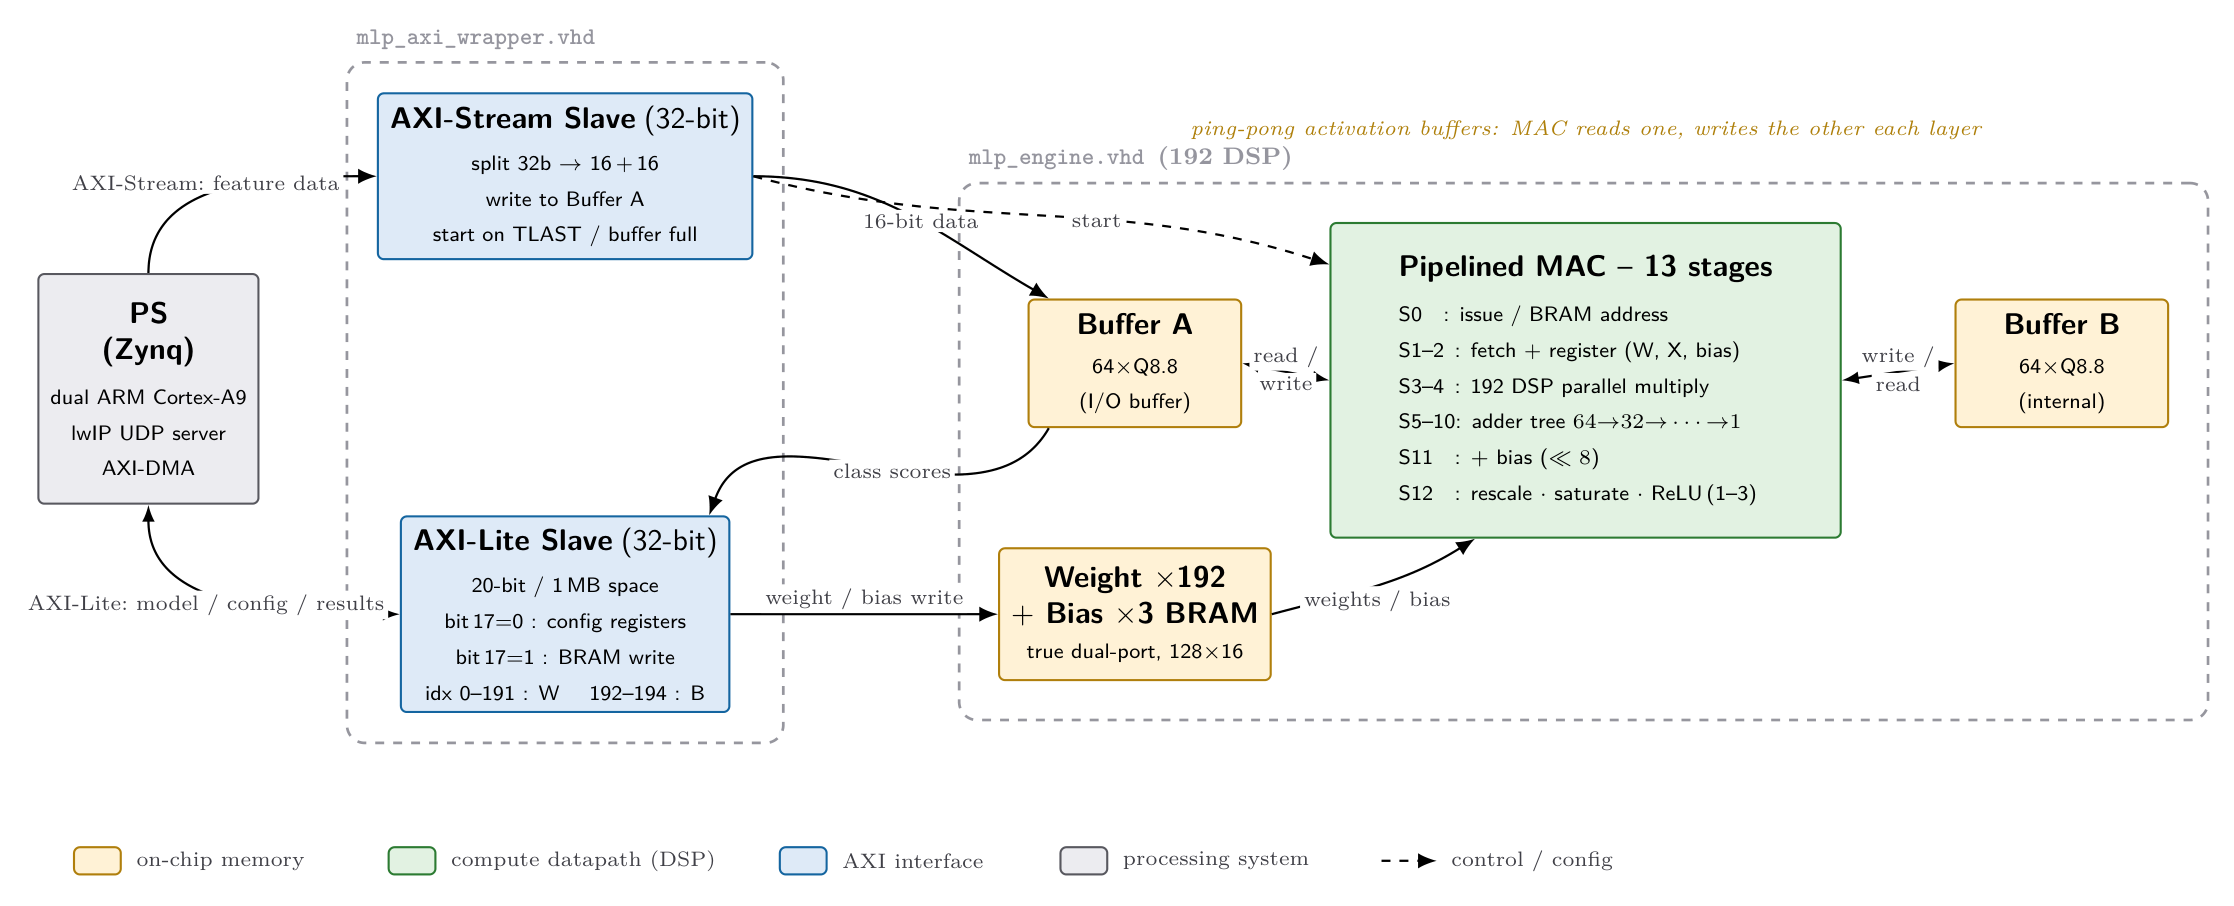
\includegraphics[width=0.92\textwidth]{figures/system_architecture.png}
\caption{System architecture of the proposed framework on the Zynq-7000 SoC.
Market data arrives over Ethernet at the PS, which forwards the prepared
feature vector to the custom \texttt{mlp\_axi\_wrapper} core through
AXI-DMA / AXI-Stream; the model parameters are loaded and the final decision
is read back over AXI-Lite. The entire inference is executed by the 13-stage
pipelined MAC engine in the PL.}
\label{fig:block_design}
\end{figure*}

\subsection{Ethernet-Enabled Data Path}
Feature packets are delivered over Ethernet to the PS, parsed, and forwarded to
the PL. Each 32-bit AXI-Stream word carries two 16-bit $Q8.8$ values, and the 40
features, zero-padded to the 64-wide datapath, are transferred as 32 stream
words on which the engine auto-starts. Table~\ref{tab:ethernet_measurement_plan}
lists the per-stage measurement points for the Ethernet-to-decision path; every
stage is instrumented and quantified over a 1{,}004{,}229-packet run in
Section~\ref{sec:eval} (Table~\ref{tab:latency_breakdown}).

\begin{table}[H]
\centering
\caption{Ethernet-enabled data path measurement plan}
\label{tab:ethernet_measurement_plan}
\begin{tabular}{p{3.2cm} p{4.2cm}}
\toprule
Metric & Description \\
\midrule
Packet receive latency & PS-side NIC-to-buffer time, $\approx$\SI{7.6}{\micro\second} \\
Packet parsing latency & Feature extraction in PS, $\approx$\SI{0.7}{\micro\second} \\
DMA transfer latency & AXI-DMA PS$\rightarrow$PL transfer, $\approx$\SI{3.7}{\micro\second} \\
MLP inference latency & PL core, \SI{768}{\nano\second} (Sec.~\ref{sec:eval}) \\
Packet-to-decision latency & Full end-to-end, $\approx$\SI{68.6}{\micro\second} \\
\bottomrule
\end{tabular}
\end{table}

\subsection{Customization Flow}
The framework is reusable across models and strategies. A user trains an MLP on
their own dataset and feature set; the trained parameters are quantized and the
on-chip weight/bias memories are regenerated, while the datapath, AXI
interfaces, and control logic are unchanged. Table~\ref{tab:customization_options}
summarizes the configurable components.

\begin{table}[H]
\centering
\caption{Customization options supported by the proposed framework}
\label{tab:customization_options}
\begin{tabular}{p{3.0cm} p{4.4cm}}
\toprule
Component & Customizable Parameters \\
\midrule
Input features & Feature vector contents and size (default 40) \\
MLP model & Retrainable weights/biases; hidden-layer sizes \\
Fixed-point format & Word/fraction split (default $Q8.8$) \\
Output decision & Class set, e.g.\ BUY / HOLD / SELL \\
Deployment flow & Automatic weight/bias memory regeneration \\
\bottomrule
\end{tabular}
\end{table}

%%%%%%%%%%%%%%%%%%%%%%%%%%%%%%%%%%%%%%%%%%%%%%%%%%%%%%%%%%%%%%%%%%%%%%%%%%%%%%%
\section{FPGA-Embedded Neural Inference Architecture}
%%%%%%%%%%%%%%%%%%%%%%%%%%%%%%%%%%%%%%%%%%%%%%%%%%%%%%%%%%%%%%%%%%%%%%%%%%%%%%%
The embedded network is an MLP with topology
$40\!\rightarrow\!64\!\rightarrow\!32\!\rightarrow\!16\!\rightarrow\!3$: a
40-dimensional input feature vector, three hidden layers with ReLU activation,
and a 3-class output (BUY/HOLD/SELL) selected by an argmax decision block.
Inference is performed entirely in hardware; no layer is offloaded to the PS.

\subsection{Fixed-Point Quantization}
The floating-point model is converted to a $Q8.8$ fixed-point representation
(8 integer, 8 fractional bits), which lowers resource usage and enables
single-cycle DSP multiplications while preserving accuracy. Weights and biases
are stored in BRAM and addressed through the AXI-Lite configuration interface.
Table~\ref{tab:quantization_eval} reports the quantization evaluation; values
known from the model study (Section~\ref{sec:eval}) are filled, the rest are to
be completed.

\begin{table}[H]
\centering
\caption{Quantization evaluation}
\label{tab:quantization_eval}
\begin{tabular}{p{3.1cm} p{4.3cm}}
\toprule
Metric & Value / Purpose \\
\midrule
Float accuracy & 61.74\% (reference model) \\
FPGA Q8.8 accuracy & 61.65\% (reference model) \\
Python Q8.8 vs float agreement & 99.93\% (macro F1 0.990) \\
Output match rate (Python Q8.8 vs FPGA) & 96.85\% (159{,}447 / 164{,}627) \\
Max absolute output error & 1.374 (mean 0.335) \\
Class change ratio (float vs Q8.8) & 0.074\% \\
\bottomrule
\end{tabular}
\end{table}

\subsection{Parallel MAC-Based Inference Core}
The inference core (\texttt{mlp\_engine}) is built around 192 DSP slices that
perform multiply-accumulate operations in parallel, organized as a 13-stage
pipeline (Fig.~\ref{fig:microarch}): one address-issue stage (S0) followed by
twelve datapath stages. Stages 1--2 read weights/inputs from BRAM
and register them; stages 3--4 perform the 192 parallel multiplications;
stages 5--10 reduce the products through a balanced $64\!\rightarrow\!1$ adder
tree; stage 11 adds the bias; and stage 12 rescales the result and applies the
ReLU activation before write-back.
Two ping-pong buffers (Buffer~A / Buffer~B) hold the inter-layer activations so
that successive layers reuse the same MAC array.

\begin{figure*}[t]
\centering
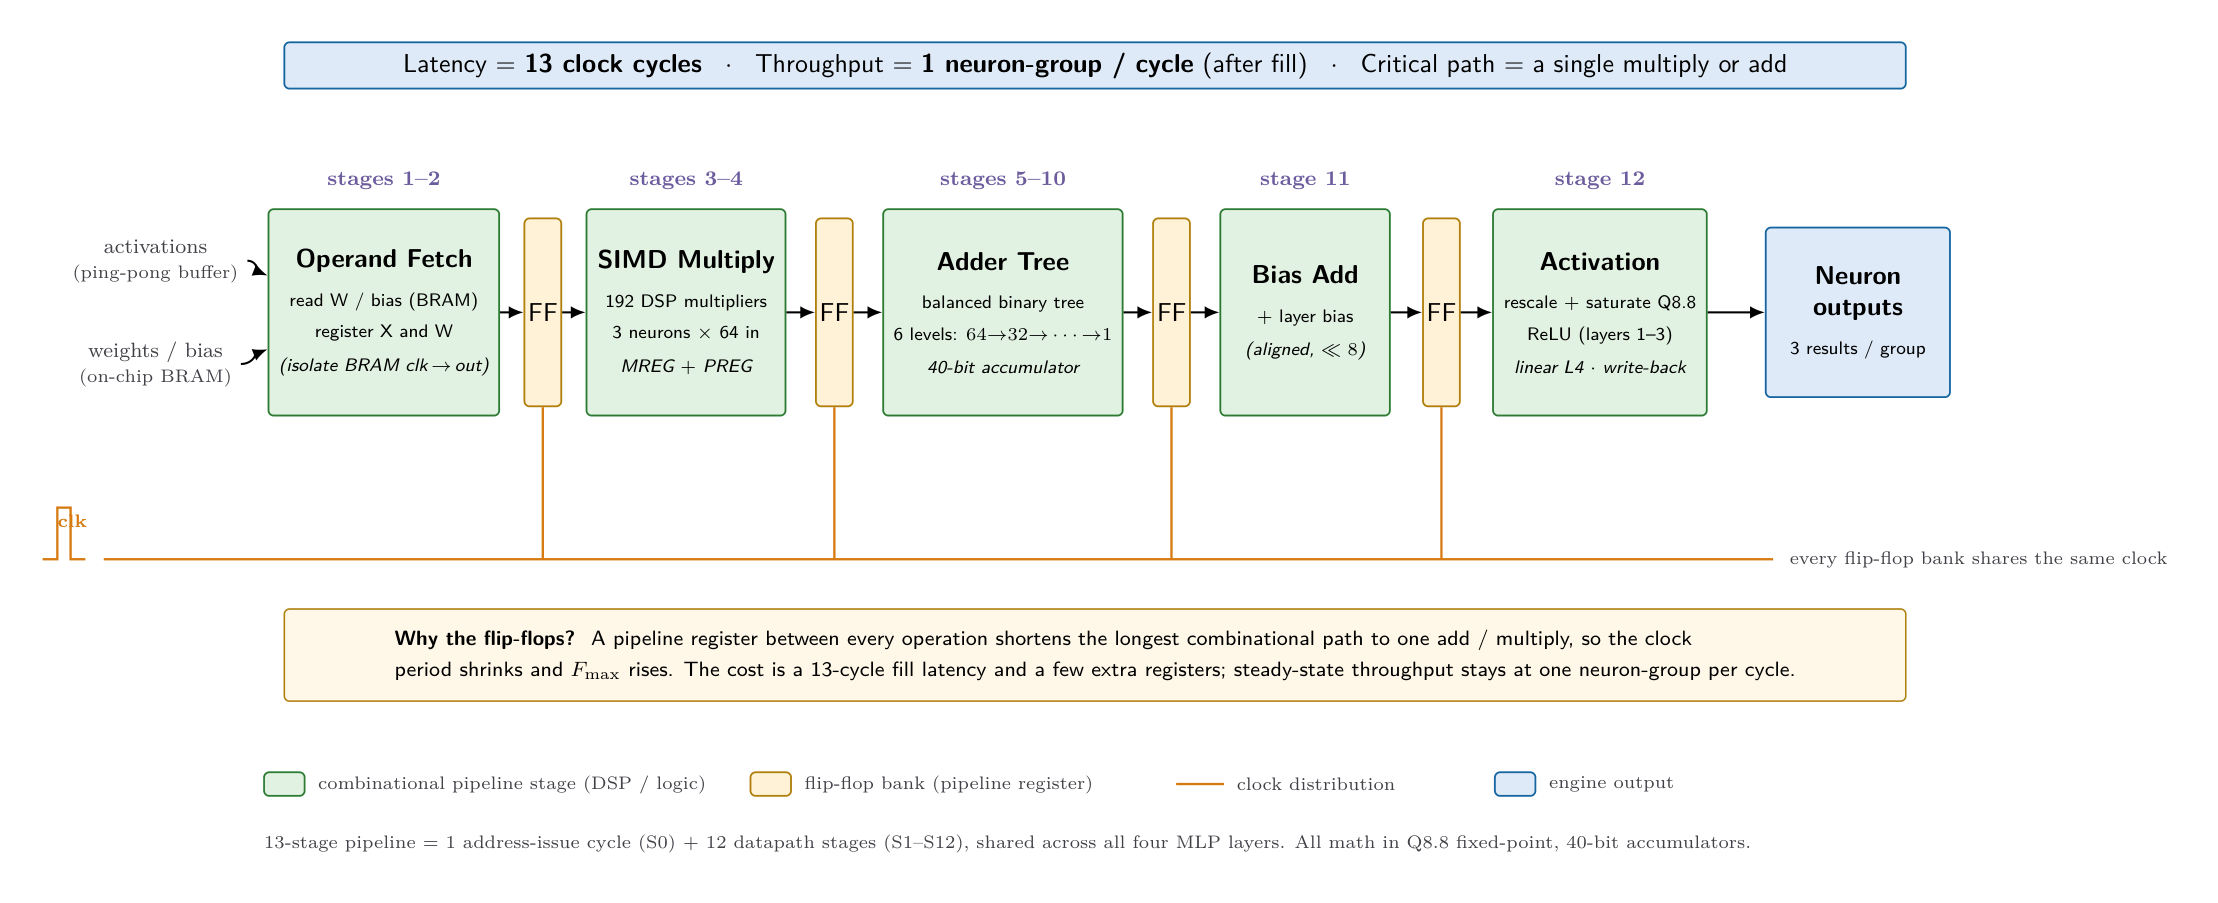
\includegraphics[width=0.92\textwidth]{figures/mlp_engine_pipeline.png}
\caption{Pipeline datapath of the hardware MLP core (\texttt{mlp\_engine}).
After the address-issue stage (S0), stages 1--2 fetch the weights, inputs, and
bias from BRAM; stages 3--4 perform the 192 parallel $Q8.8$ multiplications on
the DSP slices; stages 5--10 form the balanced $64\!\rightarrow\!1$ adder tree;
stage 11 adds the bias; and stage 12 rescales and applies the ReLU before the
result is written back to the ping-pong activation buffers. The
\texttt{mlp\_axi\_wrapper} splits each 32-bit AXI-Stream word into two 16-bit
$Q8.8$ values and triggers the engine; weights/biases reside in BRAM and are
loaded via AXI-Lite (address bit~17 selects configuration vs.\ memory).}
\label{fig:microarch}
\end{figure*}

%%%%%%%%%%%%%%%%%%%%%%%%%%%%%%%%%%%%%%%%%%%%%%%%%%%%%%%%%%%%%%%%%%%%%%%%%%%%%%%
\section{Implementation on Zynq-7000 SoC}
%%%%%%%%%%%%%%%%%%%%%%%%%%%%%%%%%%%%%%%%%%%%%%%%%%%%%%%%%%%%%%%%%%%%%%%%%%%%%%%

\subsection{Hardware/Software Partitioning}
Table~\ref{tab:hw_sw_partitioning} lists where each function is implemented.
The PS is responsible for the network interface, feature preparation, and
high-level control; the PL implements the inference core, the argmax decision,
and the debug/measurement signals.

\begin{table}[t]
\centering
\caption{Hardware/software partitioning of the proposed system}
\label{tab:hw_sw_partitioning}
\begin{tabular}{p{2.8cm} p{4.6cm}}
\toprule
Component & Implementation Location \\
\midrule
Ethernet packet reception & PS (software) \\
Feature preparation & PS (software) \\
Feature vector transfer & AXI-DMA (PS$\rightarrow$PL) \\
MLP inference & PL (hardware) \\
Argmax decision & PL (hardware) \\
Status/result registers & AXI-Lite (PS$\leftrightarrow$PL) \\
Debug signals & PL output pins \\
\bottomrule
\end{tabular}
\end{table}

\subsection{AXI-Stream and AXI-DMA Interface}
The PS prepares the feature vector and transfers it to the PL with AXI-DMA; the
\texttt{mlp\_axi\_wrapper} consumes it as an AXI-Stream slave, splitting each
32-bit word into two $Q8.8$ operands and starting the engine once a full vector
is received. Control and status (start, busy, done, result) use AXI-Lite. This
keeps the inference pipeline continuously fed without per-operand PS
intervention.

\subsection{Debug and Measurement Infrastructure}
To measure hardware timing directly, the core exports the dedicated debug
signals of Table~\ref{tab:debug_signals}. \texttt{dbg\_data\_in\_pulse} marks
the arrival of a complete feature vector, \texttt{dbg\_layer1..4\_done} pulse as
each layer finishes, and \texttt{dbg\_mlp\_busy} brackets the whole inference.
These pins are probed with an oscilloscope, so the per-layer latency is observed
on real silicon rather than estimated (Section~\ref{sec:eval}).

\begin{table}[H]
\centering
\caption{Debug signals exported for hardware latency measurement}
\label{tab:debug_signals}
\begin{tabular}{p{3.0cm} p{4.4cm}}
\toprule
Signal & Purpose \\
\midrule
\texttt{dbg\_data\_in\_pulse} & Full feature vector received \\
\texttt{dbg\_layer1\_done} & Layer~1 ($40\!\rightarrow\!64$) complete \\
\texttt{dbg\_layer2\_done} & Layer~2 ($64\!\rightarrow\!32$) complete \\
\texttt{dbg\_layer3..4\_done} & Layers 3--4 complete \\
\texttt{dbg\_mlp\_busy} & Inference in progress (decision valid on fall) \\
\bottomrule
\end{tabular}
\end{table}

%%%%%%%%%%%%%%%%%%%%%%%%%%%%%%%%%%%%%%%%%%%%%%%%%%%%%%%%%%%%%%%%%%%%%%%%%%%%%%%
\section{Experimental Evaluation}
\label{sec:eval}
%%%%%%%%%%%%%%%%%%%%%%%%%%%%%%%%%%%%%%%%%%%%%%%%%%%%%%%%%%%%%%%%%%%%%%%%%%%%%%%

\subsection{Experimental Setup}
The framework is implemented on a Xilinx Zynq-7000 SoC. A host control
application (Fig.~\ref{fig:gui}) connects to the C++ host engine, uploads the
quantized model, and streams either real CSV market data or randomized test
packets while reporting the last prediction, last latency, and processed-packet
count. Table~\ref{tab:experimental_setup} summarizes the setup.

\begin{figure}[t]
\centering
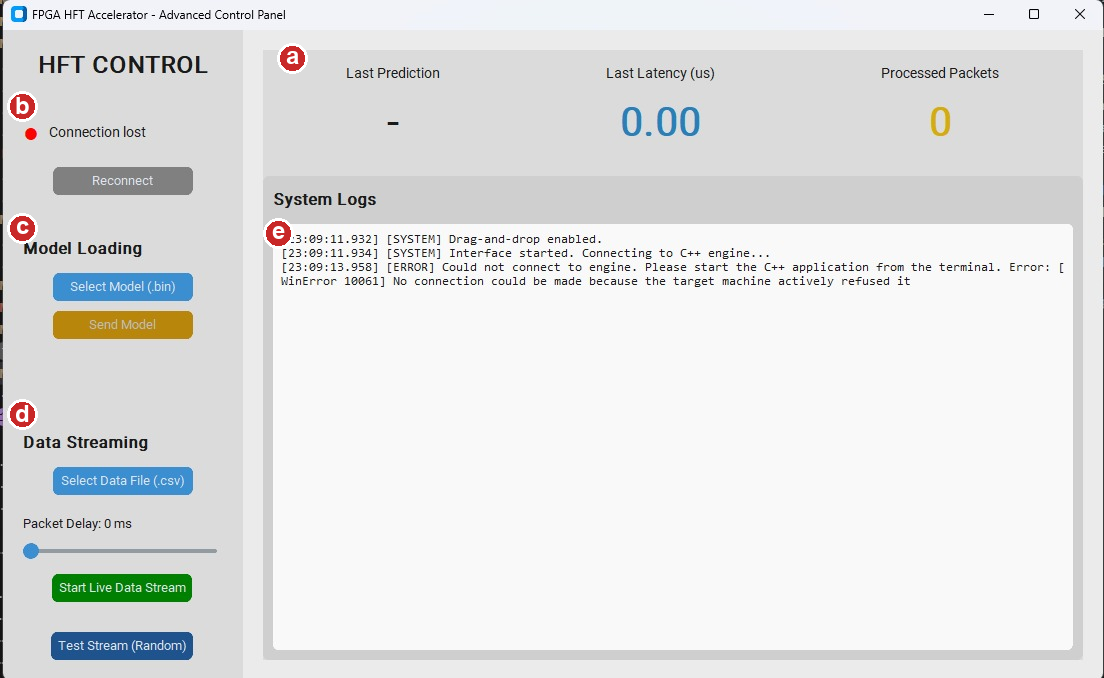
\includegraphics[width=\linewidth]{figures/host_gui_annotated.png}
\caption{Host control application used to configure, drive, and validate the
FPGA inference system. (a) Real-time dashboard showing the last predicted
decision, the last measured round-trip latency in microseconds, and the number
of processed packets. (b) Engine connection status and reconnect control,
indicating whether the host is connected to the inference engine. (c)
Model-loading panel, used to select a trained model (\texttt{.bin}) and upload
it to the board over the network. (d) Data-streaming panel, used to select a
recorded CSV dataset, set the inter-packet delay, and start either a live
stream or a randomized test stream. (e) System-log console, which reports
connection events, errors, and run-time messages during operation.}
\label{fig:gui}
\end{figure}

\begin{table}[t]
\centering
\caption{Experimental setup}
\label{tab:experimental_setup}
\begin{tabular}{p{3.1cm} p{4.3cm}}
\toprule
Item & Description \\
\midrule
FPGA platform & Xilinx Zynq-7000 SoC \\
Design language & VHDL (PL); C++/Python (PS/host) \\
Software environment & Xilinx Vivado 2025.2 \\
Data path & Ethernet $\to$ PS $\to$ AXI-DMA $\to$ AXI-Stream $\to$ PL \\
Inference core & MLP $40$-$64$-$32$-$16$-$3$, $Q8.8$, 192 DSP MACs \\
Test size & 120{,}883 inference requests (Linux end-to-end) \\
Clock frequency & \SI{125}{\mega\hertz} (PL) \\
\bottomrule
\end{tabular}
\end{table}

\subsection{Model Accuracy and Classification Performance}
Quantizing the network to $Q8.8$ and executing it on the FPGA preserves the
classification behaviour: across five trained models the FPGA accuracy tracks
the PyTorch floating-point accuracy within at most 0.22 percentage points
(Fig.~\ref{fig:model_comp}). This confirms that the fixed-point hardware path is
not merely fast but also faithful to the trained model, which is essential to
the framework claim. Table~\ref{tab:model_performance} reports the per-model
accuracies and their absolute differences; for the reference Model~A the
difference is below $0.1\%$.

\begin{figure}[H]
\centering
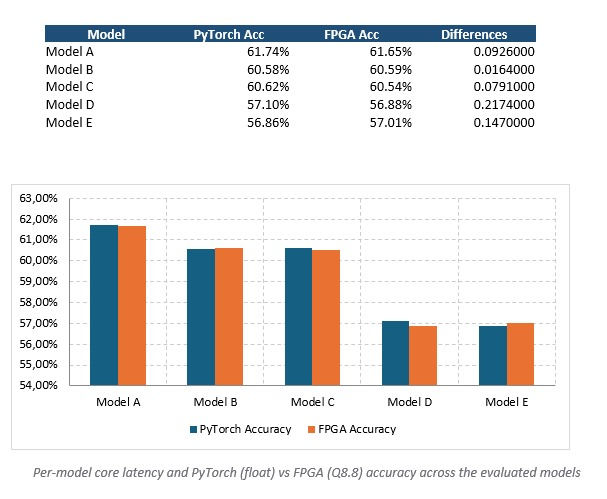
\includegraphics[width=\linewidth]{figures/model_comparison.jpeg}
\caption{PyTorch (float) vs.\ FPGA ($Q8.8$) accuracy across the five evaluated
models. The per-model absolute differences (top table) stay within 0.22
percentage points, confirming that $Q8.8$ quantization preserves the trained
model's behaviour.}
\label{fig:model_comp}
\end{figure}

\begin{table}[H]
\centering
\caption{PyTorch (float) vs.\ FPGA ($Q8.8$) accuracy for the five trained
models; the last column is the absolute accuracy difference in percentage
points.}
\label{tab:model_performance}
\begin{tabular}{lccc}
\toprule
Model & PyTorch Acc & FPGA Acc & Difference \\
\midrule
Model A & 61.74\% & 61.65\% & 0.0926 \\
Model B & 60.58\% & 60.59\% & 0.0164 \\
Model C & 60.62\% & 60.54\% & 0.0791 \\
Model D & 57.10\% & 56.88\% & 0.2174 \\
Model E & 56.86\% & 57.01\% & 0.1470 \\
\bottomrule
\end{tabular}
\end{table}

\subsection{System-Level Packet-to-Decision Latency}
Table~\ref{tab:latency_metrics} reports the measured end-to-end
packet-to-decision latency of the full FPGA system on the Linux host over
120{,}883 inference requests. Each request is a UDP round trip from the host to
the board and back, so it includes the network, the PS software, the AXI-DMA
transfer, and the PL core. The median is \SI{66.3}{\micro\second}; the pure
hardware core (Section~\ref{sec:eval}, \SI{768}{\nano\second}) is therefore
about \SI{1}{\percent} of the end-to-end time, confirming that the remaining
cost is dominated by the operating system, the network, and the PS software
rather than by the inference itself.

\begin{table}[H]
\centering
\caption{Measured end-to-end packet-to-decision latency of the FPGA system
(Linux host, 120{,}883 requests)}
\label{tab:latency_metrics}
\begin{tabular}{lc}
\toprule
Metric & Latency \\
\midrule
Minimum & \SI{50.0}{\micro\second} \\
Median & \SI{66.3}{\micro\second} \\
Mean & \SI{65.6}{\micro\second} \\
99th Percentile & \SI{79.6}{\micro\second} \\
99.9th Percentile & \SI{109.7}{\micro\second} \\
Maximum & \SI{3275.9}{\micro\second} \\
\bottomrule
\end{tabular}
\end{table}

\subsection{Software Baseline: OS-Induced Latency and Jitter}
\label{sec:osbaseline}
To show how strongly the end-to-end latency depends on the host operating
system, the same UDP round-trip run was repeated on a Linux and a Windows host.
Figure~\ref{fig:lat_hist} shows the two latency distributions.
The Linux host completes a median request in \SI{66.3}{\micro\second} (p99
\SI{79.6}{\micro\second}), whereas the Windows host needs
\SI{476.3}{\micro\second} (p99 \SI{608.7}{\micro\second}) and exhibits a much
heavier tail (p99.9 \SI{1649}{\micro\second}) and occasional timeouts. This
roughly $7\times$ difference in median latency between two hosts running the
same board and the same model illustrates exactly the operating-system
non-determinism that the deterministic PL core removes: the outliers originate
on the PS/host side, not in the pipeline, whose latency is fixed by its depth.

\begin{figure}[H]
\centering
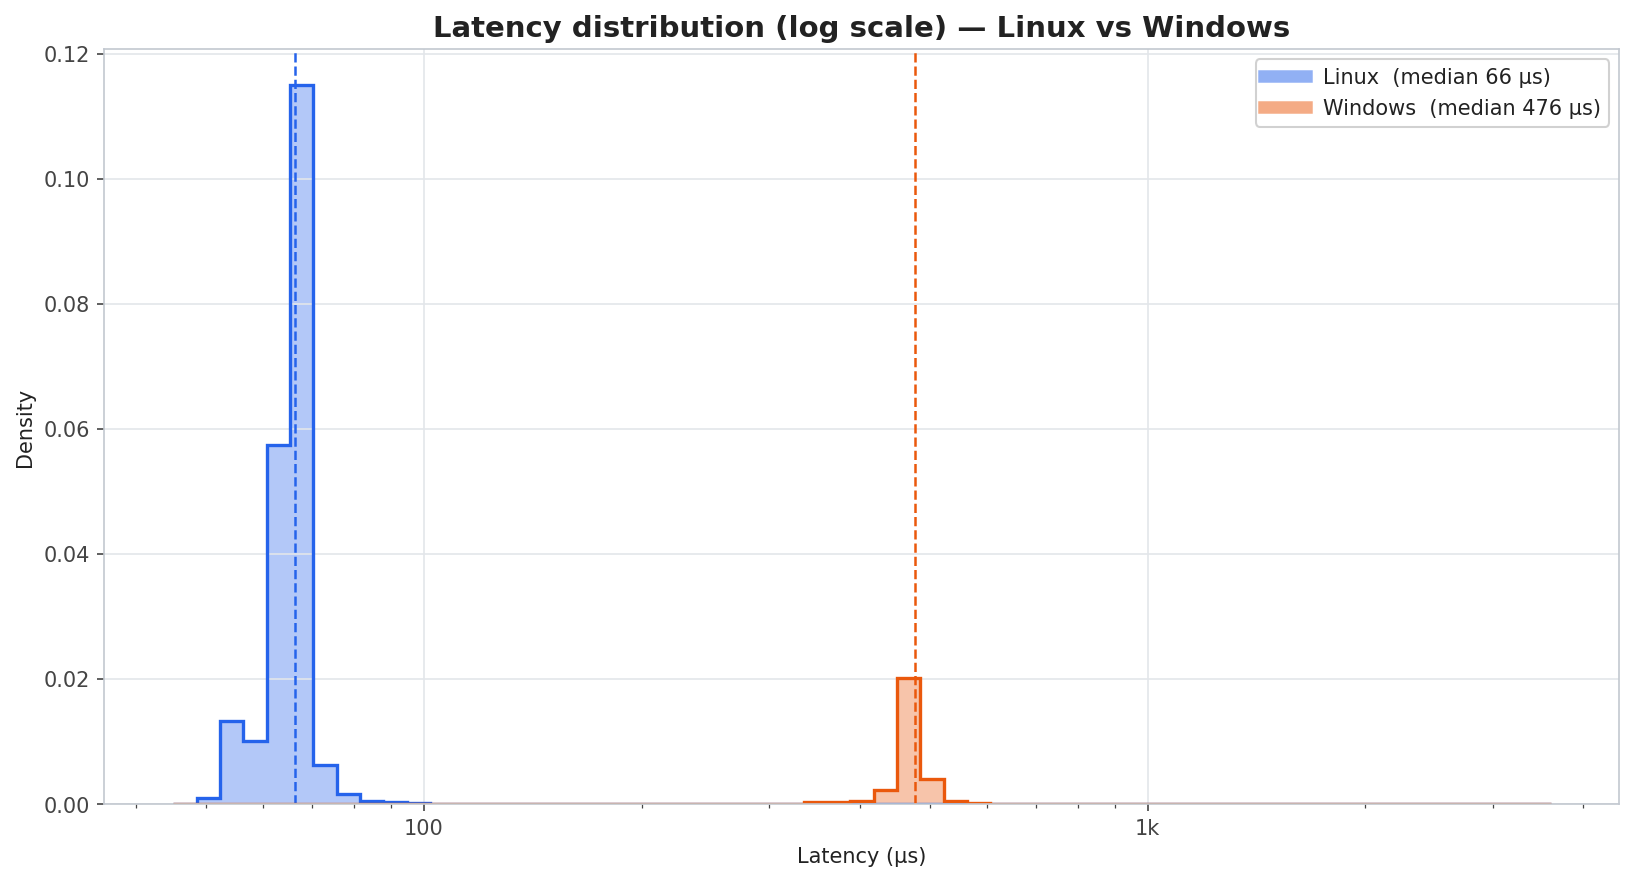
\includegraphics[width=\linewidth]{figures/lat_hist.png}
\caption{End-to-end latency distribution (log scale) on the Linux vs.\ Windows
host driving the same FPGA board. The OS-dependent gap and the heavier Windows
tail are evident.}
\label{fig:lat_hist}
\end{figure}

\subsection{Latency Breakdown}
Because each layer exposes a done pulse, the inference can be decomposed on real
hardware. Probing the debug pins with an oscilloscope yields the per-layer
inter-pulse times of Fig.~\ref{fig:scope_layer} and the total
input-to-final-done interval of Fig.~\ref{fig:scope_total}.
Table~\ref{tab:cycle_breakdown} converts these to clock cycles at
\SI{125}{\mega\hertz}. The measured per-layer times are 280, 200, 160,
and \SI{118}{\nano\second} for layers~1--4 (a sum of \SI{758}{\nano\second}),
and the measured end-to-end core interval is \SI{768}{\nano\second}; the
difference between the total and the sum of the layer times corresponds to the
input-streaming and output-decision stages that are not bracketed by the
layer-done pulses.

The full end-to-end path was then instrumented with PS-side timestamps over
1{,}004{,}229 packets (Table~\ref{tab:latency_breakdown}). The result isolates
where the time is spent: of the \SI{68.6}{\micro\second} mean host-to-decision
latency, only \SI{14.4}{\micro\second} is spent on the board (PS + PL), and the
remaining \SI{54}{\micro\second} is host-side NIC, operating-system, and wire
time. On the board, the Ethernet reception (EMAC + lwIP) dominates and is
bimodal (p50 \SI{2.6}{\micro\second} vs p99 \SI{14.2}{\micro\second}), reflecting
the phase of the polling loop relative to packet arrival, whereas the DMA,
PL compute, and readout stages are tightly bounded (sub-microsecond to a few
microseconds, with p99 within a few percent of the median). This confirms the
central claim: the deterministic hardware core is a negligible and jitter-free
fraction of the end-to-end latency, and the remaining cost is host- and
network-side software, which a hardware Ethernet MAC in the PL would remove.

\begin{figure}[H]
\centering
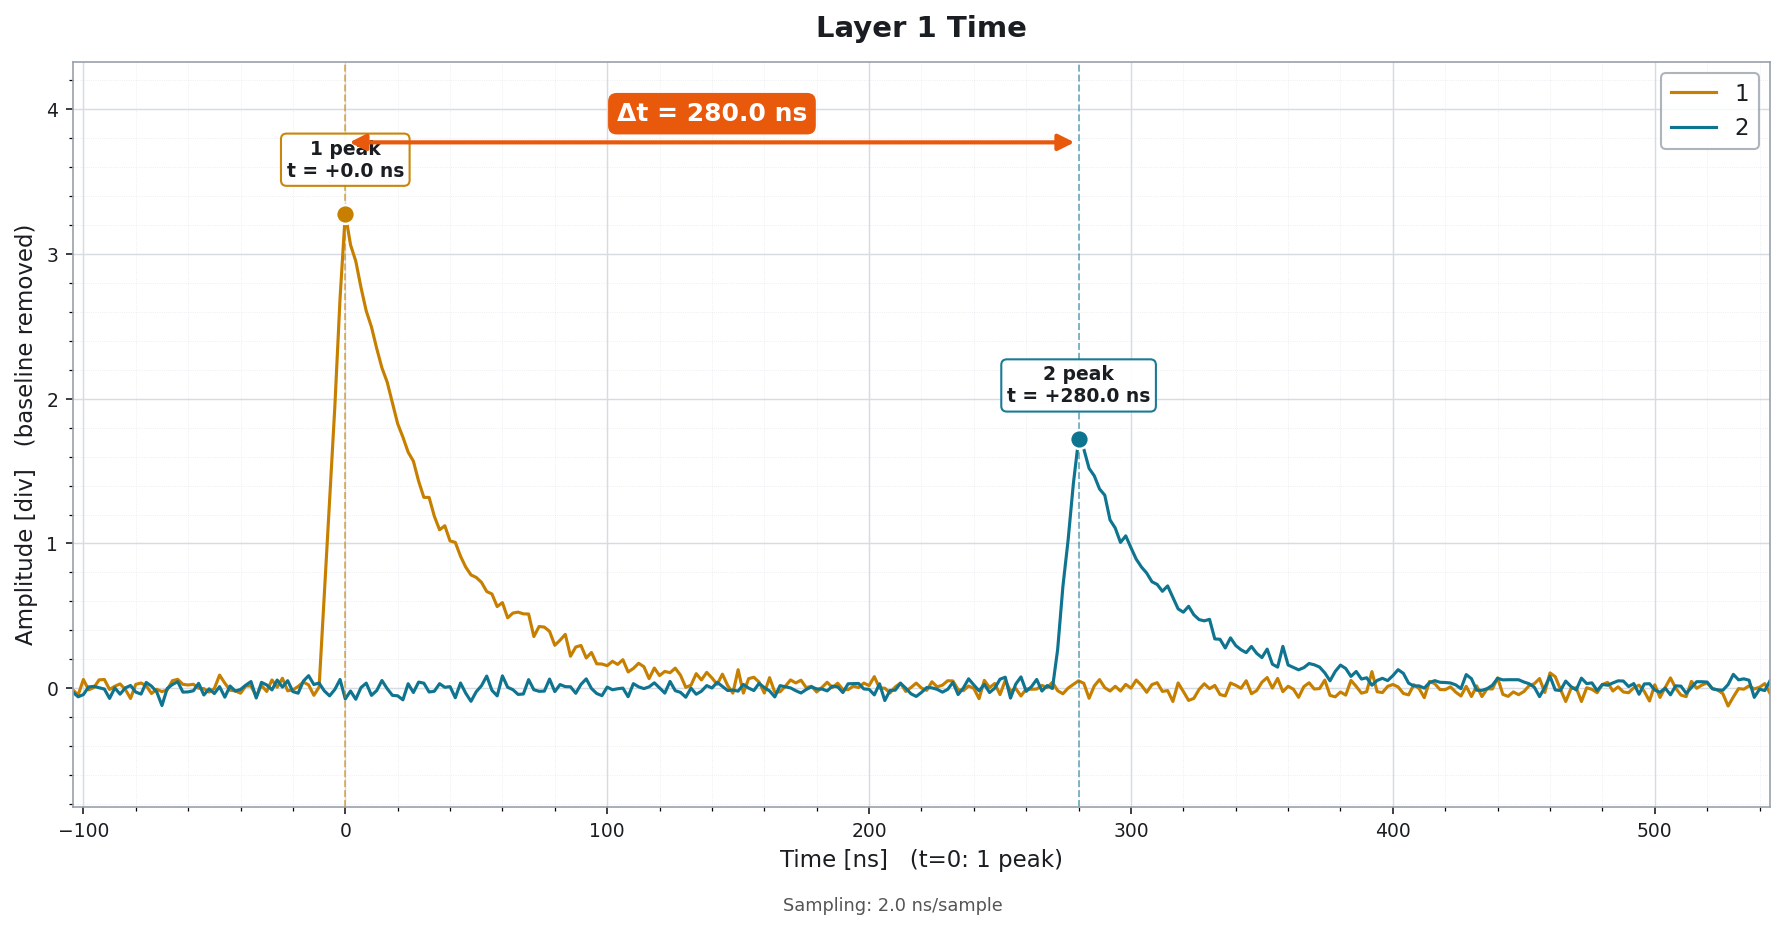
\includegraphics[width=0.49\linewidth]{figures/scope_layer1.png}\hfill
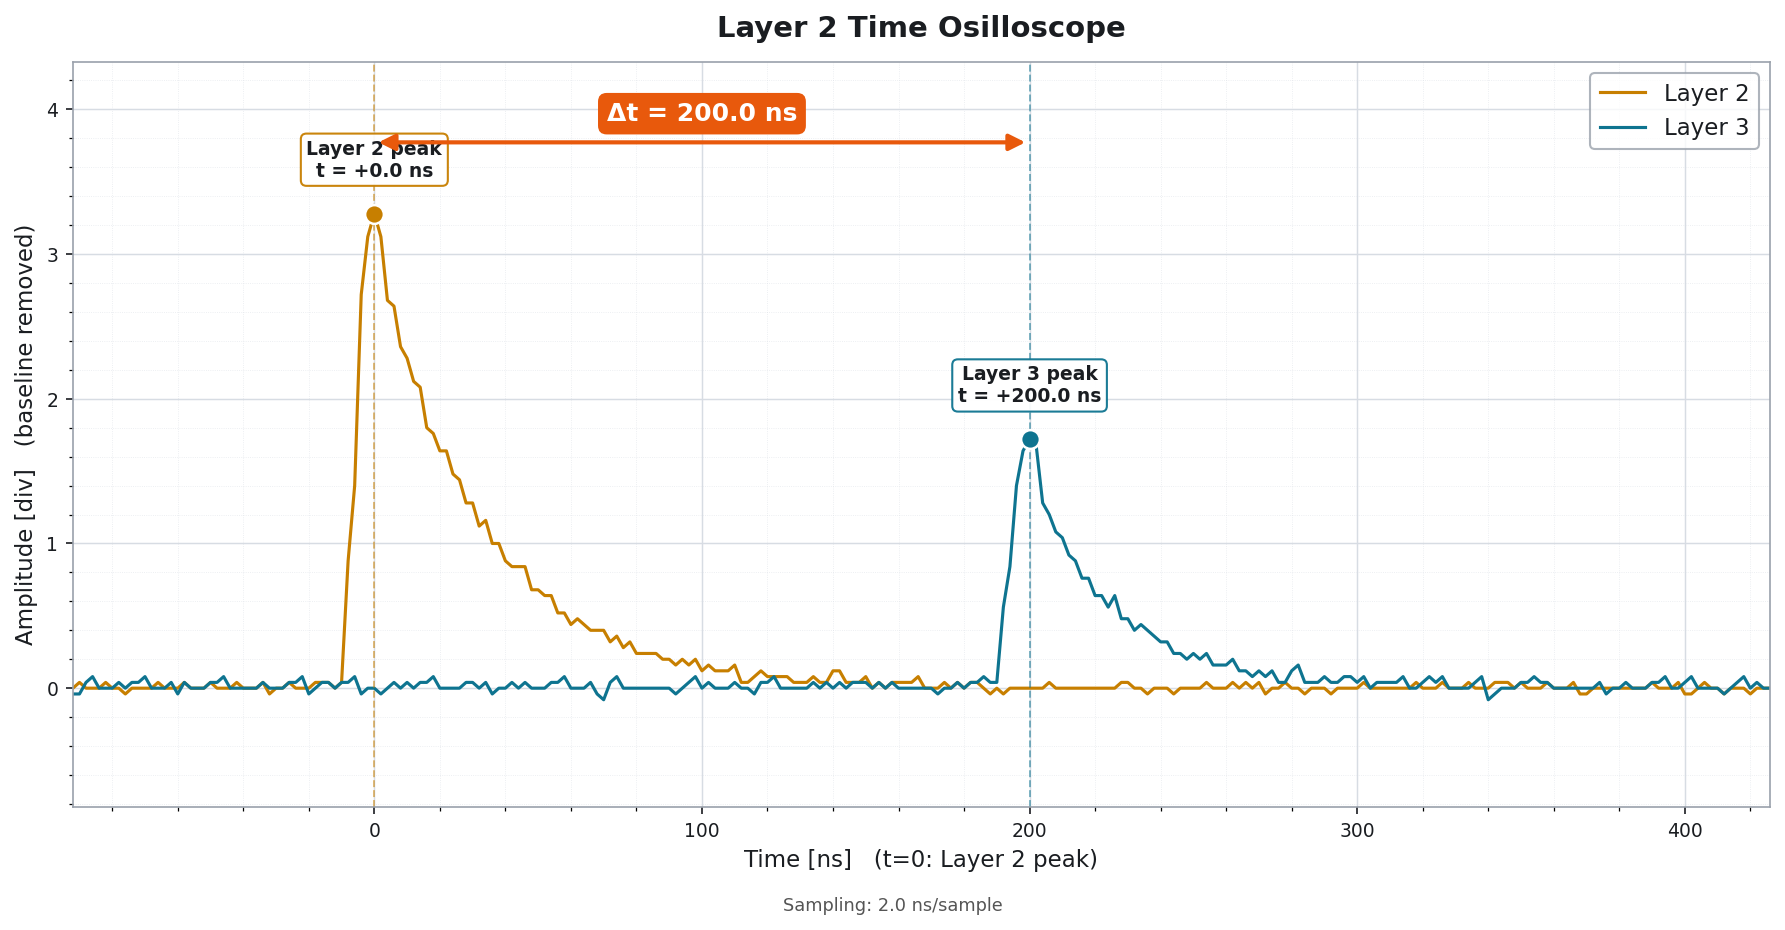
\includegraphics[width=0.49\linewidth]{figures/scope_layer2.png}\\[3pt]
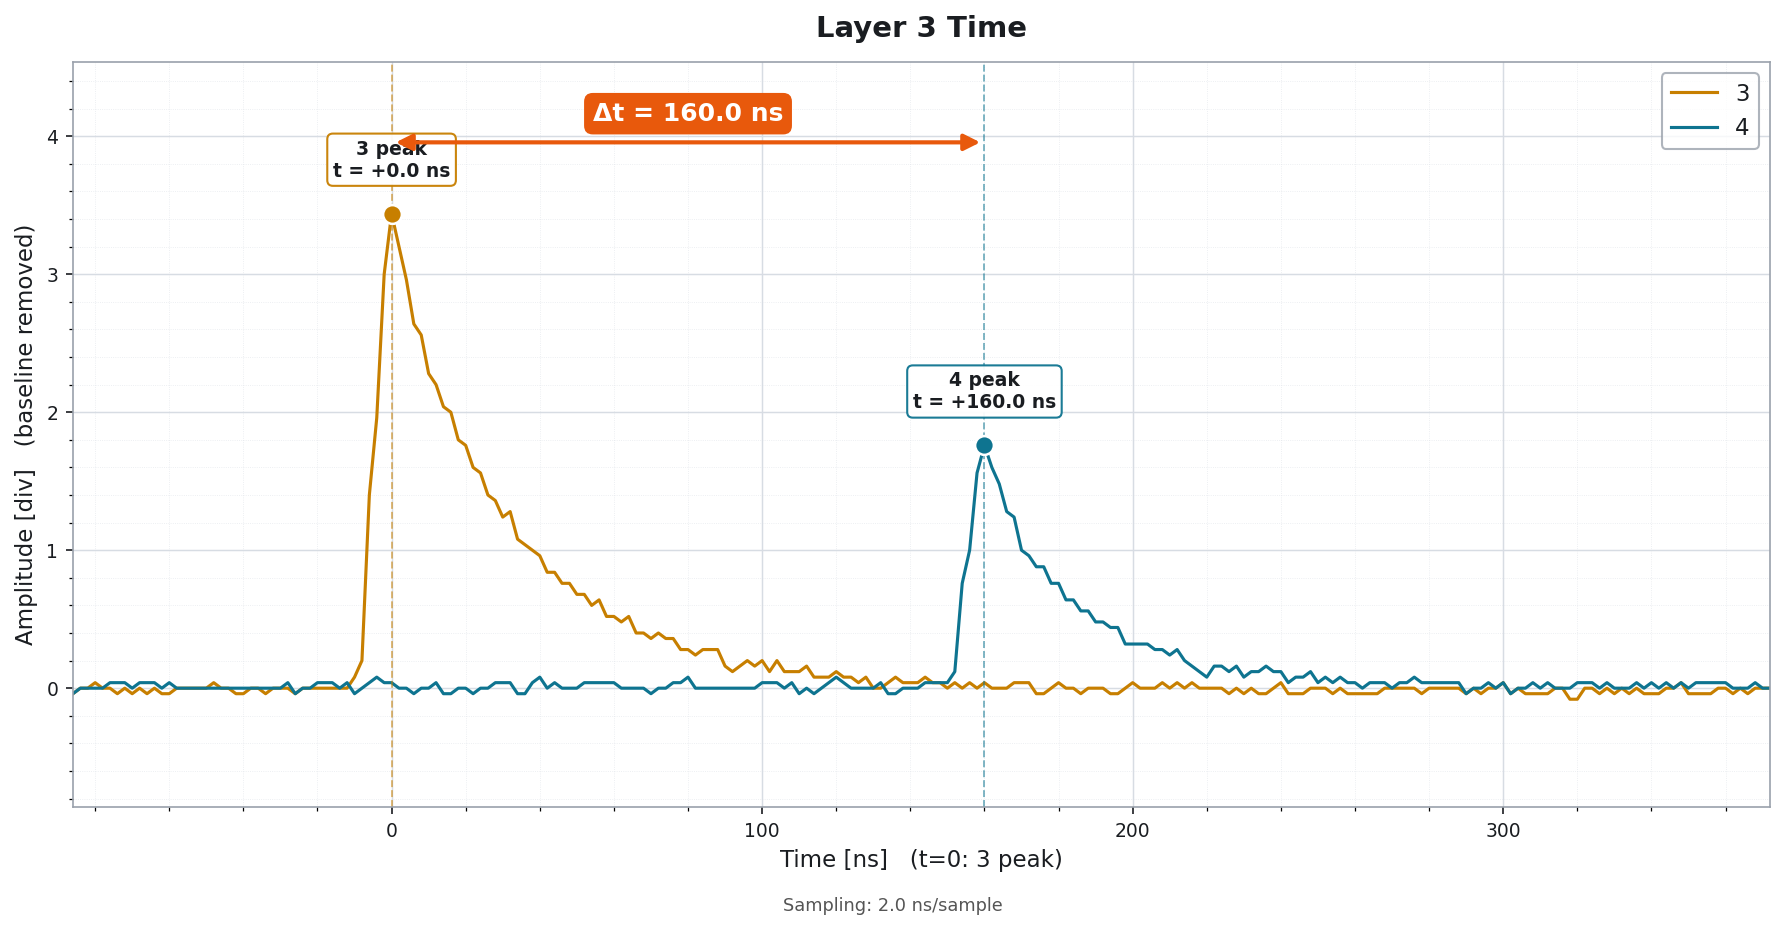
\includegraphics[width=0.49\linewidth]{figures/scope_layer3.png}\hfill
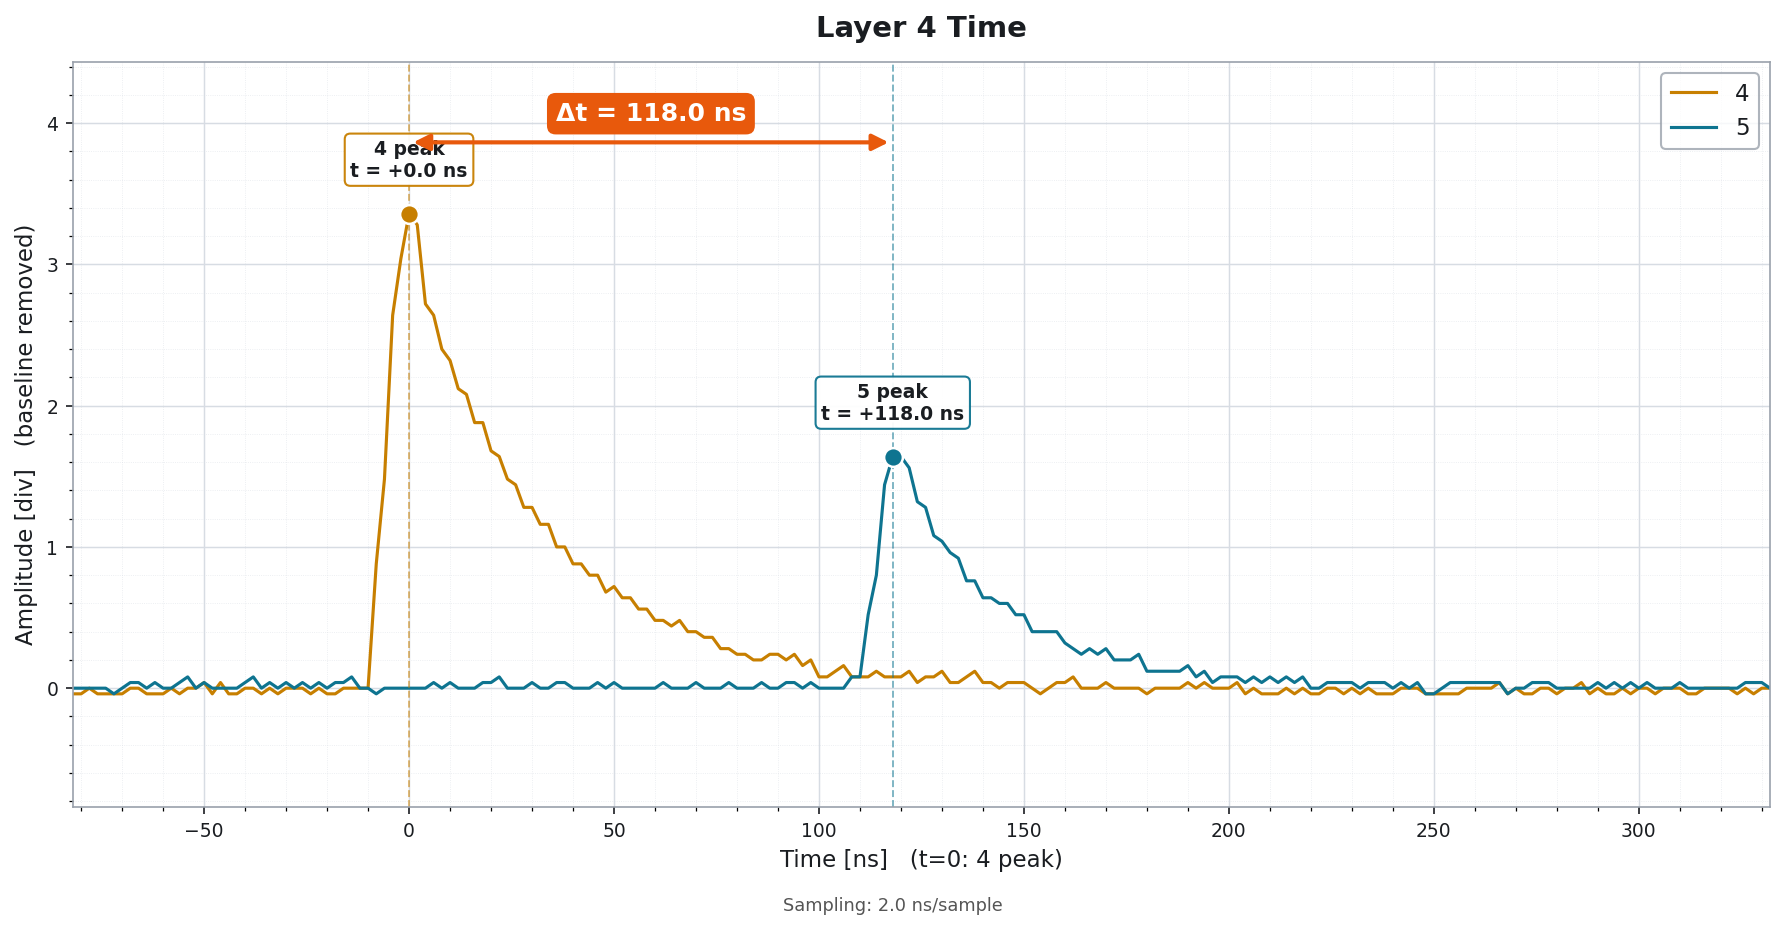
\includegraphics[width=0.49\linewidth]{figures/scope_layer4.png}
\caption{Oscilloscope captures of consecutive layer-done debug pulses; each
inter-pulse interval directly measures one layer's processing time. Top-left to
bottom-right: layer~1 (\SI{280}{\nano\second}), layer~2
(\SI{200}{\nano\second}), layer~3 (\SI{160}{\nano\second}), layer~4
(\SI{118}{\nano\second}).}
\label{fig:scope_layer}
\end{figure}

\begin{figure}[H]
\centering
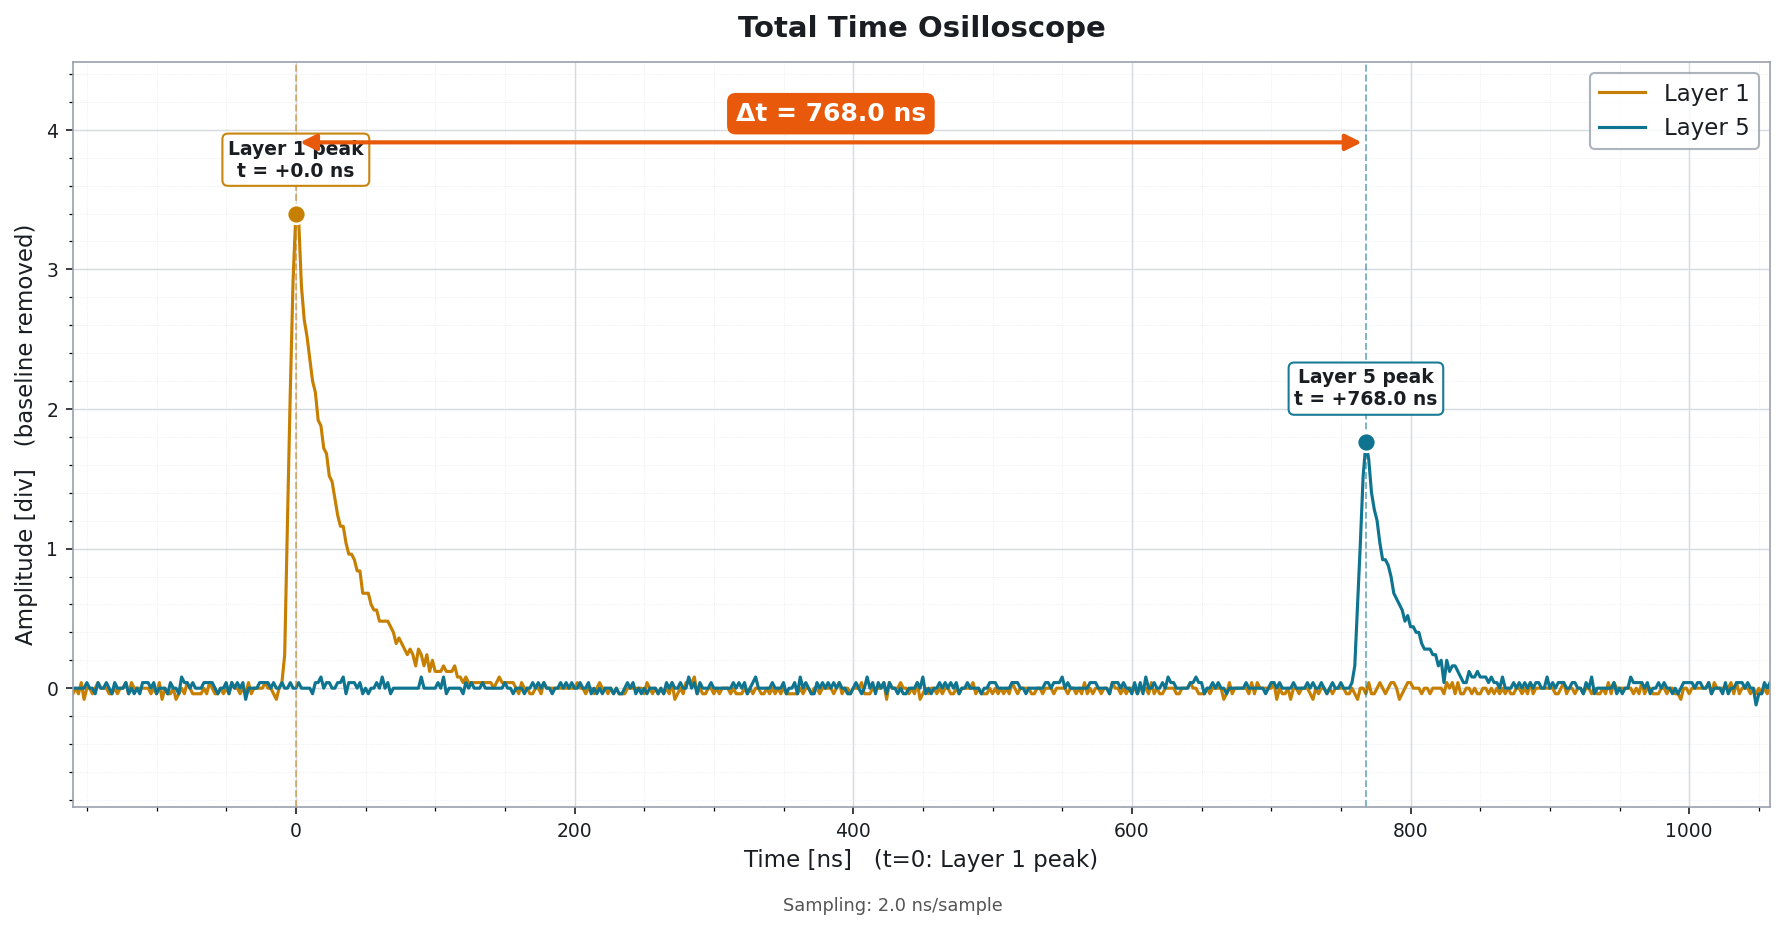
\includegraphics[width=\linewidth]{figures/scope_total.png}
\caption{Oscilloscope capture of the first and last debug pulses of an
inference, measuring the total hardware-core interval
($\Delta t = \SI{768}{\nano\second}$).}
\label{fig:scope_total}
\end{figure}

\begin{table*}[t]
\centering
\caption{Latency breakdown from Ethernet packet to trading decision, over a
1{,}004{,}229-packet run (all values in $\mu$s)}
\label{tab:latency_breakdown}
\begin{tabular}{p{4.6cm} p{1.5cm} p{2.4cm} p{4.4cm}}
\toprule
Stage & Mean & p50 / p99 & Measurement Method \\
\midrule
Ethernet packet reception (EMAC + lwIP) & 7.59 & 2.57 / 14.18 & PS timestamping (bimodal) \\
Packet parsing and feature preparation & 0.70 & 0.69 / 0.86 & PS timestamping \\
AXI-DMA transfer to PL & 3.70 & 3.70 / 3.78 & PS/PL counters \\
AXI-Stream receive + MLP core (PL) & 1.46 & 1.46 / 1.72 & \texttt{dbg} pins (core \SI{768}{\nano\second}) \\
Result readout & 0.96 & 0.96 / 0.97 & AXI-Lite \\
\midrule
Board subtotal (PS + PL) & 14.40 & 9.41 / 21.03 & On-board sum \\
Host end-to-end & 68.56 & 68.50 / 80.92 & Host round trip \\
\bottomrule
\end{tabular}
\end{table*}

\begin{table}[H]
\centering
\caption{FPGA per-layer breakdown of the MLP core (\SI{125}{\mega\hertz})}
\label{tab:cycle_breakdown}
\begin{tabular}{lcc}
\toprule
Stage & Measured Time & Measured Cycles \\
\midrule
Layer 1 ($40\!\rightarrow\!64$) & \SI{280}{\nano\second} & 35 \\
Layer 2 ($64\!\rightarrow\!32$) & \SI{200}{\nano\second} & 25 \\
Layer 3 ($32\!\rightarrow\!16$) & \SI{160}{\nano\second} & 20 \\
Layer 4 ($16\!\rightarrow\!3$)  & \SI{118}{\nano\second} & 15 \\
Total core (in$\rightarrow$done) & \SI{768}{\nano\second} & 96 \\
\bottomrule
\end{tabular}
\end{table}

\subsection{Pure FPGA-Core Latency Measurement}
The oscilloscope measurements establish that the pure hardware inference
completes in \SI{768}{\nano\second}, i.e.\ below one microsecond and
deterministic, in contrast to the tens-to-hundreds of microseconds and heavy
tails of the software baseline (Section~\ref{sec:osbaseline}). This is the core
quantitative argument for embedding the network in the PL.

\subsection{FPGA Resource Utilization}
Table~\ref{tab:resource_utilization} reports the post-implementation resource
usage on the Zynq-7000, and Fig.~\ref{fig:util_table} shows the detailed
utilization report. The design is DSP-bound (\SI{87.3}{\percent}), as
expected for a MAC-parallel core, while LUT and FF usage stay low
(\SI{27.3}{\percent} and \SI{10.8}{\percent}) and BRAM usage is
\SI{70.4}{\percent}, leaving room for larger feature
sets or networks. Timing closes at the \SI{125}{\mega\hertz} target with
positive slack on all checks (Fig.~\ref{fig:timing}: setup WNS
\SI{0.118}{\nano\second}, hold WHS \SI{0.042}{\nano\second}, pulse width WPWS
\SI{3.02}{\nano\second}; zero failing endpoints). The implemented on-chip power
is \SI{2.781}{\watt} (Fig.~\ref{fig:power}), with a junction temperature of
\SI{57.1}{\celsius} and a \SI{27.9}{\celsius} thermal margin. It is
dominated by the PS (PS7, \SI{1.535}{\watt}); the PL logic, DSP, and BRAM
together account for well under \SI{1}{\watt}, consistent with a low-cost
embedded deployment.

\begin{table}[H]
\centering
\caption{FPGA resource utilization of the proposed MLP framework (Zynq-7000)}
\label{tab:resource_utilization}
\begin{tabular}{lccc}
\toprule
Resource & Used & Available & Utilization \\
\midrule
LUTs & 14{,}523 & 53{,}200 & 27.30\% \\
Flip-Flops & 11{,}472 & 106{,}400 & 10.78\% \\
DSPs & 192 & 220 & 87.27\% \\
BRAMs & 98.5 & 140 & 70.36\% \\
Fmax & $\approx$\SI{127}{\mega\hertz} & -- & at \SI{125}{\mega\hertz} target \\
WNS & \SI{0.118}{\nano\second} & -- & positive (met) \\
\bottomrule
\end{tabular}
\end{table}

\begin{figure}[t]
\centering
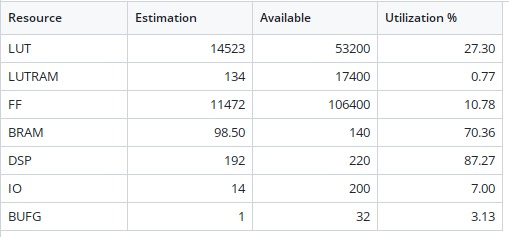
\includegraphics[width=\linewidth]{figures/util_table.jpeg}
\caption{Detailed post-implementation utilization report (used vs.\ available):
LUT 14{,}523/53{,}200, FF 11{,}472/106{,}400, BRAM 98.5/140, DSP 192/220.}
\label{fig:util_table}
\end{figure}

\begin{figure}[t]
\centering
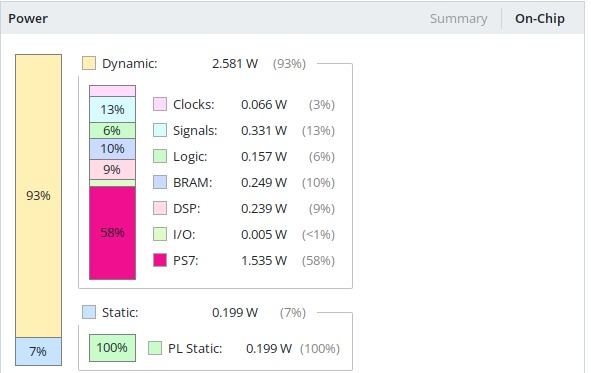
\includegraphics[width=\linewidth]{figures/power_onchip.jpeg}
\caption{On-chip power breakdown (\SI{2.781}{\watt} total on-chip power,
junction temperature \SI{57.1}{\celsius}, \SI{27.9}{\celsius} thermal margin).
Dynamic power is dominated by the PS (PS7, \SI{1.535}{\watt}); the PL
contributions (signals, logic, BRAM, DSP) remain modest.}
\label{fig:power}
\end{figure}

\begin{figure}[t]
\centering
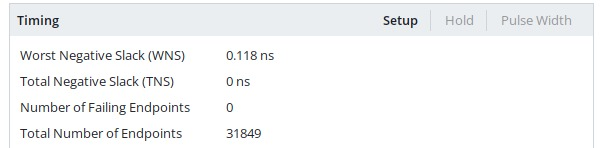
\includegraphics[width=0.88\linewidth]{figures/timing_setup.jpeg}
\caption{Post-implementation setup-timing closure on the Zynq-7000 at the
\SI{125}{\mega\hertz} target: WNS \SI{0.118}{\nano\second} with zero failing
endpoints. The hold (WHS \SI{0.042}{\nano\second}) and pulse-width
(WPWS \SI{3.02}{\nano\second}) checks are also met.}
\label{fig:timing}
\end{figure}

\subsection{Low-Cost Platform Evaluation}

\begin{table*}[t]
\centering
\caption{Cost-oriented comparison of possible inference platforms}
\label{tab:cost_comparison}
\begin{tabular}{p{3.0cm} p{2.4cm} p{2.8cm} p{2.0cm} p{2.3cm} p{2.2cm}}
\toprule
Platform & Platform Class & Acceleration Type & Cost Level & Latency & Power \\
\midrule
CPU-based system & General-purpose & Software & Low--Med & 66--476\,$\mu$s (OS-dep.) & Moderate--high \\
GPU-based system & General-purpose & Batched SIMD & High & High per query (batch-oriented) & High \\
High-end FPGA card~\cite{sparknoc} & Datacenter & Hardware & Very high & 337.2\,GOP/s (throughput) & $\approx$\SI{7.6}{\watt} \\
Proposed Zynq system & Embedded SoC & Hardware (PL) & Low & \SI{768}{\nano\second} core & \SI{2.78}{\watt} \\
\bottomrule
\end{tabular}
\end{table*}

Table~\ref{tab:cost_comparison} positions the proposed system against CPU-,
GPU-, and high-end-FPGA-card alternatives. The key point is qualitative: a
sub-microsecond, deterministic inference path is obtained on an accessible Zynq
SoC rather than on an expensive accelerator card, while the software (CPU)
options pay both higher latency and substantial OS jitter
(Section~\ref{sec:osbaseline}). As a representative high-end FPGA accelerator,
the SparkNoC design on an Intel Arria 10 GX1150 card reaches 337.2 GOP/s at
44.48 GOP/s/W (about \SI{7.6}{\watt} of compute power)~\cite{sparknoc}; it
delivers high throughput but requires a data-center-class board, whereas the
proposed system targets sub-microsecond single-inference latency on a low-cost
embedded SoC.

\subsection{Customization and Scalability}
The same datapath serves different trained models by regenerating only the
fixed-point weight/bias memories; the topology, AXI interfaces, and control
logic are unchanged. Consequently the five evaluated models share one identical
hardware configuration and the same resource footprint: only the weights, and
hence the accuracy (Table~\ref{tab:model_performance}), differ. This is the core
framework property, one reconfigurable core hosts any model that fits the
192-DSP budget, without re-synthesis.

%%%%%%%%%%%%%%%%%%%%%%%%%%%%%%%%%%%%%%%%%%%%%%%%%%%%%%%%%%%%%%%%%%%%%%%%%%%%%%%
\section{Discussion}
%%%%%%%%%%%%%%%%%%%%%%%%%%%%%%%%%%%%%%%%%%%%%%%%%%%%%%%%%%%%%%%%%%%%%%%%%%%%%%%
The results support three observations. First, embedding the network in the PL
makes the core latency a property of the pipeline rather than of the operating
system: the measured core latency is \SI{768}{\nano\second} and deterministic,
whereas the end-to-end host path around it varies from \SI{66}{} to
\SI{476}{\micro\second} in median across operating systems and shows heavy tails. Second, $Q8.8$ quantization is essentially
accuracy-neutral here (at most 0.22 percentage points across five models), so
the speed-up does not cost predictive quality. Third, the design fits a low-cost Zynq-7000 at \SI{2.78}{\watt} with
positive timing slack, so the approach does not depend on premium accelerator
hardware. The instrumented per-stage breakdown
(Table~\ref{tab:latency_breakdown}) further shows that only
\SI{14.4}{\micro\second} of the \SI{68.6}{\micro\second} end-to-end latency is
spent on the board, so the main remaining limitation is the host- and
network-side software path; moving the Ethernet stack into the PL is the clearest
next step.

%%%%%%%%%%%%%%%%%%%%%%%%%%%%%%%%%%%%%%%%%%%%%%%%%%%%%%%%%%%%%%%%%%%%%%%%%%%%%%%
\section{Conclusion}
%%%%%%%%%%%%%%%%%%%%%%%%%%%%%%%%%%%%%%%%%%%%%%%%%%%%%%%%%%%%%%%%%%%%%%%%%%%%%%%
We presented an Ethernet-enabled, customizable MLP inference framework embedded
in the programmable logic of a low-cost Zynq-7000 SoC for high-frequency
trading. Feature vectors are delivered over Ethernet and streamed to the PL via
AXI-DMA / AXI-Stream, while a 192-DSP, 13-stage pipelined core performs the
$Q8.8$ inference in \SI{768}{\nano\second} with deterministic timing and
floating-point-equivalent accuracy, using \SI{27}{\percent} of the LUTs and
\SI{87}{\percent} of the DSPs at \SI{2.78}{\watt}. Because features, network
shape, fixed-point format, and decision classes are configurable, the system is
a reusable FPGA-embedded AI inference framework, demonstrated on an HFT task.
Future work includes runtime weight loading, larger models, and direct PL
Ethernet MAC integration to remove the host- and network-side software that
now dominates the measured end-to-end latency.

%%%%%%%%%%%%%%%%%%%%%%%%%%%%%%%%%%%%%%%%%%%%%%%%%%%%%%%%%%%%%%%%%%%%%%%%%%%%%%%
\section*{Acknowledgments}
%%%%%%%%%%%%%%%%%%%%%%%%%%%%%%%%%%%%%%%%%%%%%%%%%%%%%%%%%%%%%%%%%%%%%%%%%%%%%%%
\writinggap[1.0cm]

%%%%%%%%%%%%%%%%%%%%%%%%%%%%%%%%%%%%%%%%%%%%%%%%%%%%%%%%%%%%%%%%%%%%%%%%%%%%%%%
% REFERENCES
%%%%%%%%%%%%%%%%%%%%%%%%%%%%%%%%%%%%%%%%%%%%%%%%%%%%%%%%%%%%%%%%%%%%%%%%%%%%%%%
\bibliographystyle{elsarticle-num}
\bibliography{references}

\end{document}
